\documentclass{article}

\usepackage{fancyhdr}
\usepackage{extramarks}
\usepackage{amsmath}
\usepackage{amsthm}
\usepackage{amsfonts}
\usepackage{tikz}
\usepackage[plain]{algorithm}
\usepackage{algpseudocode}
\usepackage{url}
\usepackage{listings}
\usepackage{xcolor}
\usepackage{hyperref}
\usepackage{graphicx}
\usepackage{placeins}
\usepackage{float}
\usepackage[utf8]{inputenc}
\usepackage{booktabs}
\usepackage{fontawesome5}

\graphicspath{{images/}}

% Define custom colors
\definecolor{codegreen}{rgb}{0,0.6,0}
\definecolor{codegray}{rgb}{0.5,0.5,0.5}
\definecolor{codepurple}{rgb}{0.58,0,0.82}
\definecolor{backcolour}{rgb}{0.95,0.95,0.92}

% Setup the style
\lstdefinestyle{mystyle}{
    backgroundcolor=\color{backcolour},
    commentstyle=\color{codegreen},
    keywordstyle=\color{magenta},
    numberstyle=\tiny\color{codegray},
    stringstyle=\color{codepurple},
    basicstyle=\ttfamily\footnotesize,
    breakatwhitespace=false,
    breaklines=true,
    captionpos=b,
    keepspaces=true,
    numbers=left,
    numbersep=5pt,
    showspaces=false,
    showstringspaces=false,
    showtabs=false,
    tabsize=2
}
\lstset{style=mystyle}

\usetikzlibrary{automata,positioning}

%
% Basic Document Settings
%
\topmargin=-0.45in
\evensidemargin=0in
\oddsidemargin=0in
\textwidth=6.5in
\textheight=9.0in
\headsep=0.25in

\linespread{1.1}

\pagestyle{fancy}
\lhead{\hmwkAuthorName}
\chead{\hmwkClass\ (\hmwkClassInstructor\ \hmwkClassTime): \hmwkTitle}
\rhead{\firstxmark}
\lfoot{\lastxmark}
\cfoot{\thepage}

\renewcommand\headrulewidth{0.4pt}
\renewcommand\footrulewidth{0.4pt}

\setlength\parindent{0pt}

%
% Create Problem Sections
%
\newcommand{\enterProblemHeader}[1]{
    \nobreak\extramarks{}{Problem \arabic{#1} continued on next page\ldots}\nobreak{}
    \nobreak\extramarks{Problem \arabic{#1} (continued)}{Problem \arabic{#1} continued on next page\ldots}\nobreak{}
}

\newcommand{\exitProblemHeader}[1]{
    \nobreak\extramarks{Problem \arabic{#1} (continued)}{Problem \arabic{#1} continued on next page\ldots}\nobreak{}
    \stepcounter{#1}
    \nobreak\extramarks{Problem \arabic{#1}}{}\nobreak{}
}

\setcounter{secnumdepth}{0}
\newcounter{partCounter}
\newcounter{homeworkProblemCounter}
\setcounter{homeworkProblemCounter}{1}
\nobreak\extramarks{Problem \arabic{homeworkProblemCounter}}{}\nobreak{}

%
% Homework Problem Environment
%
\newenvironment{homeworkProblem}[1][-1]{
    \ifnum#1>0
        \setcounter{homeworkProblemCounter}{#1}
    \fi
    \section{Question \arabic{homeworkProblemCounter}}
    \setcounter{partCounter}{1}
    \enterProblemHeader{homeworkProblemCounter}
}{
    \exitProblemHeader{homeworkProblemCounter}
}

%
% Homework Details
%
\newcommand{\hmwkTitle}{Homework\ \#4}
\newcommand{\hmwkDueDate}{9th April 2026}
\newcommand{\hmwkClass}{IEOR 4578}
\newcommand{\hmwkClassTime}{}
\newcommand{\hmwkClassInstructor}{}
\newcommand{\hmwkAuthorName}{\textbf{Luca Barattini - UNI: LB3656}}

% GitHub repository links
\newcommand{\hmwkNbURL}{https://github.com/lucabarattini/IEOR-4578/tree/main/HW4}
\newcommand{\hmwkPdfURL}{https://github.com/lucabarattini/IEOR-4578/blob/main/HW4/HW4.pdf}

%
% Title Page
%
\hypersetup{
    colorlinks=true,
    linkcolor=blue,
    filecolor=magenta,
    urlcolor=blue,
}

\title{
    \vspace{2in}
    \textmd{\textbf{\hmwkClass:\ \hmwkTitle}}\\
    \normalsize\vspace{0.1in}\small{Due\ on\ \hmwkDueDate}\\
    \vspace{0.1in}\large{\textit{\hmwkClassInstructor\ \hmwkClassTime}}\\
    \vspace{0.25in}
    \large{
        \textbf{Code Repositories:} \\
        \vspace{0.1in}
        \href{\hmwkNbURL}{\faGithub \ Jupyter Notebooks} \hspace{0.5in}
        \href{\hmwkPdfURL}{\faGithub \ Exported PDF}
    }
    \vspace{3in}
}

\author{\hmwkAuthorName}
\date{}

\renewcommand{\part}[1]{\textbf{\large Part \Alph{partCounter}}\stepcounter{partCounter}\\}

%
% Various Helper Commands
%
\newcommand{\solution}{\textbf{\large Solution}}

\begin{document}

\maketitle
\pagebreak

% ==========================================
% QUESTION 1
% ==========================================
\begin{homeworkProblem}

\textbf{Run the OLS related code shared in the ``GLM.py'' file for the \texttt{us\_macro\_quarterly.xlsx} data: [Points 30]}
\begin{itemize}
    \item Explain the model summary when all the data is fit. Discuss R-squared, Df Residuals, Df Model, Method, F-statistic, Prob (F-statistic), Log-Likelihood, AIC, BIC, Coef, Std err, t, and $P > |t|$.
    \item Compute t-value for each parameter including the constant using the equation provided in the lecture.
    \item Run the function \texttt{t\_score\_probability} to find the probability of the null hypothesis for each parameter's t-value including the constant. And list which ones are statistically significant.
    \item Using $t_{\alpha/2}$, where $\alpha = 0.05$, compute lower and upper CI for the constant, $\beta_4$, and $\beta_6$.
    \item Run with the train-test split based on the ordering and compare the results of the test with the above model fitted on the entire data.
    \item Run all three variations of ANOVA and discuss results on SSR, df\_diff, ss\_diff, df\_resid, F and $\Pr(>F)$.
    \item Submit appropriately labeled visuals.
\end{itemize}

The target is \texttt{PCECTPI} (Personal Consumption Expenditures Chain-type Price Index). The regressors are \texttt{JAPAN\_IP}, \texttt{GS10}, \texttt{GS1}, \texttt{TB3MS}, \texttt{UNRATE}, \texttt{EXUSUK}. After \texttt{sm.add\_constant} the coefficient layout is $\beta_0 = $ const, $\beta_1 = $ \texttt{JAPAN\_IP} (\texttt{x1}), $\beta_2 = $ \texttt{GS10} (\texttt{x2}), $\beta_3 = $ \texttt{GS1} (\texttt{x3}), $\beta_4 = $ \texttt{TB3MS} (\texttt{x4}), $\beta_5 = $ \texttt{UNRATE} (\texttt{x5}), $\beta_6 = $ \texttt{EXUSUK} (\texttt{x6}).

\hrulefill

\subsection*{Part a) Full-Sample OLS Summary}

\begin{lstlisting}[language=Python, title={Python Console Output: Full-Sample OLS Summary}]
                            OLS Regression Results
==============================================================================
Dep. Variable:                      y   R-squared:                       0.956
Model:                            OLS   Adj. R-squared:                  0.954
Method:                 Least Squares   F-statistic:                     766.5
Date:                Fri, 10 Apr 2026   Prob (F-statistic):          3.40e-141
Time:                        17:54:09   Log-Likelihood:                -716.96
No. Observations:                 220   AIC:                             1448.
Df Residuals:                     213   BIC:                             1472.
Df Model:                           6
Covariance Type:            nonrobust
==============================================================================
                 coef    std err          t      P>|t|      [0.025      0.975]
------------------------------------------------------------------------------
const         19.8404      7.586      2.615      0.010       4.888      34.793
x1             0.8143      0.031     26.350      0.000       0.753       0.875
x2            -7.6966      0.824     -9.337      0.000      -9.322      -6.072
x3             6.2944      1.840      3.421      0.001       2.668       9.921
x4            -3.1825      1.547     -2.057      0.041      -6.232      -0.133
x5             3.8759      0.375     10.338      0.000       3.137       4.615
x6            -7.6557      2.202     -3.476      0.001    -11.997      -3.314
==============================================================================
\end{lstlisting}

\textbf{Discussion of each summary statistic:}
\begin{itemize}
    \item \textbf{Method = Least Squares.} The closed-form OLS solution $\hat{\beta} = (X^\top X)^{-1} X^\top y$ is used, no iterative optimizer.
    \item \textbf{No. Observations = 220, Df Model = 6, Df Residuals = 213.} We have $n = 220$ quarters and $k = 7$ parameters (6 regressors plus the intercept), so residual degrees of freedom $= n - k = 213$. ``Df Model'' counts regressors excluding the intercept.
    \item \textbf{R-squared = 0.956.} The six macro regressors jointly explain $95.6\%$ of the variance in \texttt{PCECTPI}. The Adjusted R-squared ($0.954$) penalises for the six extra parameters but is almost identical, confirming there is no over-fitting from the added regressors.
    \item \textbf{F-statistic = 766.5, Prob(F-statistic) = 3.40e-141.} Tests the joint null that all six slope coefficients are zero. The p-value is effectively zero, so we overwhelmingly reject the null: the regressors jointly carry real information about \texttt{PCECTPI}.
    \item \textbf{Log-Likelihood = $-716.96$.} The log of the joint Gaussian likelihood at the MLE. On its own it has no scale, it is only meaningful when comparing nested models.
    \item \textbf{AIC = 1448, BIC = 1472.} Penalised fit criteria ($\text{AIC} = 2k - 2\ln L$, $\text{BIC} = k\ln n - 2\ln L$). Lower is better, and BIC is stricter on model complexity.
    \item \textbf{Coef / Std err / t / P>|t|.} Per-coefficient statistics. Every regressor is significant at $\alpha = 0.05$: the largest p-value is $0.041$ for \texttt{TB3MS} ($\beta_4$), and the intercept is borderline at $0.010$. \texttt{JAPAN\_IP} has by far the largest t-statistic ($26.35$), making Japanese industrial production the single most informative regressor for US consumption prices in this model.
\end{itemize}

\subsection*{Part b) Manual t-Values}

From lecture,
$$
t_i = \frac{\hat{\beta}_i}{\mathrm{SE}(\hat{\beta}_i)}, \qquad
\mathrm{SE}(\hat{\beta}_i) = \sqrt{\hat{\sigma}^2 \left[(X^\top X)^{-1}\right]_{ii}}, \qquad
\hat{\sigma}^2 = \frac{\mathrm{RSS}}{n-k}.
$$

\begin{lstlisting}[language=Python, title={Python Console Output: Manual vs. Statsmodels t-values}]
n = 220,  k = 7,  dof = n-k = 213
RSS = 8722.021811,  sigma^2_hat = 40.948459

Parameter         Coef  SE (manual)  SE (statsmodels)   t (manual)  t (statsmodels)
    const    19.840410     7.585775          7.585775     2.615476         2.615476
 JAPAN_IP     0.814323     0.030905          0.030905    26.349530        26.349530
     GS10    -7.696645     0.824352          0.824352    -9.336602        -9.336602
      GS1     6.294430     1.839874          1.839874     3.421121         3.421121
    TB3MS    -3.182478     1.547065          1.547065    -2.057107        -2.057107
   UNRATE     3.875867     0.374901          0.374901    10.338381        10.338381
   EXUSUK    -7.655680     2.202423          2.202423    -3.476026        -3.476026
\end{lstlisting}

\textbf{Conclusion:}\\
The manually-computed standard errors and t-values match \texttt{statsmodels} to every printed digit, validating the formula from lecture.

\subsection*{Part c) Probability of the Null Hypothesis via \texttt{t\_score\_probability}}

\begin{lstlisting}[language=Python, title={Python Console Output: p-values at alpha = 0.05}]
Parameter         Coef      t-value  p-value (manual)  p-value (statsmodels)  Significant
    const    19.840410     2.615476          0.009548               0.009548          Yes
 JAPAN_IP     0.814323    26.349530          0.000000               0.000000          Yes
     GS10    -7.696645    -9.336602          0.000000               0.000000          Yes
      GS1     6.294430     3.421121          0.000748               0.000748          Yes
    TB3MS    -3.182478    -2.057107          0.040894               0.040894          Yes
   UNRATE     3.875867    10.338381          0.000000               0.000000          Yes
   EXUSUK    -7.655680    -3.476026          0.000617               0.000617          Yes

>>> Significant at alpha=0.05 : ['const', 'JAPAN_IP', 'GS10', 'GS1', 'TB3MS', 'UNRATE', 'EXUSUK']
>>> NOT significant at alpha=0.05: []
\end{lstlisting}

\textbf{Conclusion:}\\
At $\alpha = 0.05$, \textbf{every single parameter}, including the intercept, rejects its null hypothesis ($H_0 : \beta_i = 0$). The weakest evidence is for $\beta_4 = $ \texttt{TB3MS} ($p = 0.0409$), the strongest for $\beta_1 = $ \texttt{JAPAN\_IP} ($p \approx 0$).

\subsection*{Part d) 95\% Confidence Intervals for the Constant, $\beta_4$, and $\beta_6$}

With $\alpha = 0.05$ and $\mathrm{dof} = n - k = 213$, the critical value is $t_{\alpha/2,\,213} = 1.9712$. The CI is
$$\hat{\beta}_i \;\pm\; t_{\alpha/2,\,n-k} \cdot \mathrm{SE}(\hat{\beta}_i).$$

\begin{lstlisting}[language=Python, title={Python Console Output: 95\% Confidence Intervals}]
t_(alpha/2, dof=213) = 1.971164  (alpha = 0.05)

  Parameter         Coef           SE  CI 95% lower  CI 95% upper
 const (b0)    19.840410     7.585775      4.887605     34.793216
 TB3MS (b4)    -3.182478     1.547065     -6.231996     -0.132960
EXUSUK (b6)    -7.655680     2.202423    -11.997017     -3.314343
\end{lstlisting}

\textbf{Conclusion:}\\
None of the three intervals straddles zero, so at $95\%$ confidence each of $\beta_0$, $\beta_4$, and $\beta_6$ is non-zero. \texttt{TB3MS} barely clears the upper bound ($-0.133$), consistent with its marginal p-value of $0.041$.

\subsection*{Part e) Ordered 80/20 Train-Test Split}

Since \texttt{us\_macro\_quarterly.xlsx} is a time series, the ordering matters: the first 176 rows are used as training data and the remaining 44 rows are held out as test, exactly as in \texttt{GLM.py}.

\vspace{0.5em}
\begin{center}
\begin{tabular}{lrrrrrr}
\toprule
\textbf{Model} & $R^2$ & \textbf{Adj $R^2$} & \textbf{AIC} & \textbf{BIC} & \textbf{In-sample RMSE} & \textbf{Test RMSE} \\
\midrule
Full-sample (all rows) & 0.9557 & 0.9545 & 1447.9283 & 1471.6837 & 6.2965 & n/a \\
Train-only (first 176) & 0.9382 & 0.9360 & 1143.5909 & 1165.7842 & 5.9902 & 14.4276 \\
\bottomrule
\end{tabular}
\end{center}
\vspace{0.5em}

\begin{lstlisting}[language=Python, title={Python Console Output: Train-Only OLS Summary}]
                            OLS Regression Results
==============================================================================
Dep. Variable:                      y   R-squared:                       0.938
Model:                            OLS   Adj. R-squared:                  0.936
Method:                 Least Squares   F-statistic:                     427.4
Date:                Fri, 10 Apr 2026   Prob (F-statistic):           2.34e-99
Time:                        17:54:09   Log-Likelihood:                -564.80
No. Observations:                 176   AIC:                             1144.
Df Residuals:                     169   BIC:                             1166.
Df Model:                           6
Covariance Type:            nonrobust
==============================================================================
                 coef    std err          t      P>|t|      [0.025      0.975]
------------------------------------------------------------------------------
const         31.9781      8.376      3.818      0.000      15.444      48.513
x1             0.7024      0.040     17.674      0.000       0.624       0.781
x2            -4.5460      1.059     -4.291      0.000      -6.637      -2.454
x3             3.8655      1.948      1.984      0.049       0.020       7.711
x4            -2.2058      1.577     -1.399      0.164      -5.318       0.907
x5             1.5490      0.560      2.766      0.006       0.443       2.655
x6            -9.8304      2.472     -3.976      0.000     -14.711      -4.950
==============================================================================
\end{lstlisting}

\textbf{Conclusion:}\\
The train-only model achieves in-sample $R^2 = 0.938$ but its out-of-sample RMSE on the last 44 quarters is $14.43$, more than twice the in-sample RMSE of $5.99$. The jump confirms that PCECTPI drifts materially outside the 1959 to 2002 training window, and also that \texttt{TB3MS} loses significance once the 2003 to 2013 quarters are excluded (its p-value moves from $0.041$ to $0.164$). The full-sample fit is noticeably more favourable on AIC/BIC because it uses 44 additional observations that happen to carry most of the post-crisis price movement.

\subsection*{Part f) Three Variations of ANOVA}

\begin{lstlisting}[language=Python, title={Python Console Output: ANOVA 1 -- Full vs Intercept-Only}]
========================================================================
ANOVA 1 -- Full model vs Intercept-only (null) model
========================================================================
   df_resid            ssr  df_diff        ss_diff          F         Pr(>F)
0     219.0  197043.064310      0.0            NaN        NaN            NaN
1     213.0    8722.021811      6.0  188321.042498  766.49625  3.402699e-141
\end{lstlisting}

\begin{lstlisting}[language=Python, title={Python Console Output: ANOVA 2 -- Reduced (JAPAN\_IP, UNRATE, EXUSUK) vs Full}]
========================================================================
ANOVA 2 -- Reduced (const, JAPAN_IP, UNRATE, EXUSUK) vs Full
========================================================================
   df_resid           ssr  df_diff       ss_diff           F        Pr(>F)
0     216.0  29145.446498      0.0           NaN         NaN           NaN
1     213.0   8722.021811      3.0  20423.424686  166.253099  1.549676e-55
\end{lstlisting}

\begin{lstlisting}[language=Python, title={Python Console Output: ANOVA 3 -- Full vs Itself}]
========================================================================
ANOVA 3 -- Full model vs itself
========================================================================
   df_resid          ssr  df_diff  ss_diff   F  Pr(>F)
0     213.0  8722.021811      0.0      NaN NaN     NaN
1     213.0  8722.021811     -0.0     -0.0 NaN     NaN
\end{lstlisting}

\textbf{Discussion:}
\begin{itemize}
    \item \textbf{ANOVA 1.}\\
    Compares the full model to the intercept-only null ($y = \bar{y}$). The null model has $\mathrm{SSR} = 197{,}043$ with $219$ residual df, and the full model drives $\mathrm{SSR}$ down to $8{,}722$ with $213$ residual df. The extra sum of squares $\mathrm{ss\_diff} = 188{,}321$ is explained by spending $\mathrm{df\_diff} = 6$ extra parameters. $F = 766.50$ with $p = 3.4 \times 10^{-141}$. The F-statistic here equals the headline F in \texttt{summary()}, and the joint null that all slopes are zero is decisively rejected.

    \item \textbf{ANOVA 2.}\\
    Compares a reduced model containing only (const, \texttt{JAPAN\_IP}, \texttt{UNRATE}, \texttt{EXUSUK}) against the full model, testing whether the three interest-rate variables (\texttt{GS10}, \texttt{GS1}, \texttt{TB3MS}) carry information beyond the reduced set. The reduced model has $\mathrm{SSR} = 29{,}145$ with $216$ residual df, and adding the three rates drops $\mathrm{SSR}$ to $8{,}722$ ($\mathrm{ss\_diff} = 20{,}423$) at the cost of $\mathrm{df\_diff} = 3$. The F-statistic $F = 166.25$ with $p = 1.5 \times 10^{-55}$ rejects the null that those three coefficients are jointly zero. The interest-rate block is highly informative even after controlling for Japanese industrial production, unemployment, and the GBP/USD exchange rate.

    \item \textbf{ANOVA 3.}\\
    Compares the full model to itself. $\mathrm{ss\_diff} = 0$, $\mathrm{df\_diff} = 0$, and $F$ is therefore undefined (\texttt{NaN}). The test is only a structural sanity check, confirming the nested-model machinery is wired correctly.
\end{itemize}

\subsection*{Part g) Visuals}

\begin{figure}[H]
     \centering
     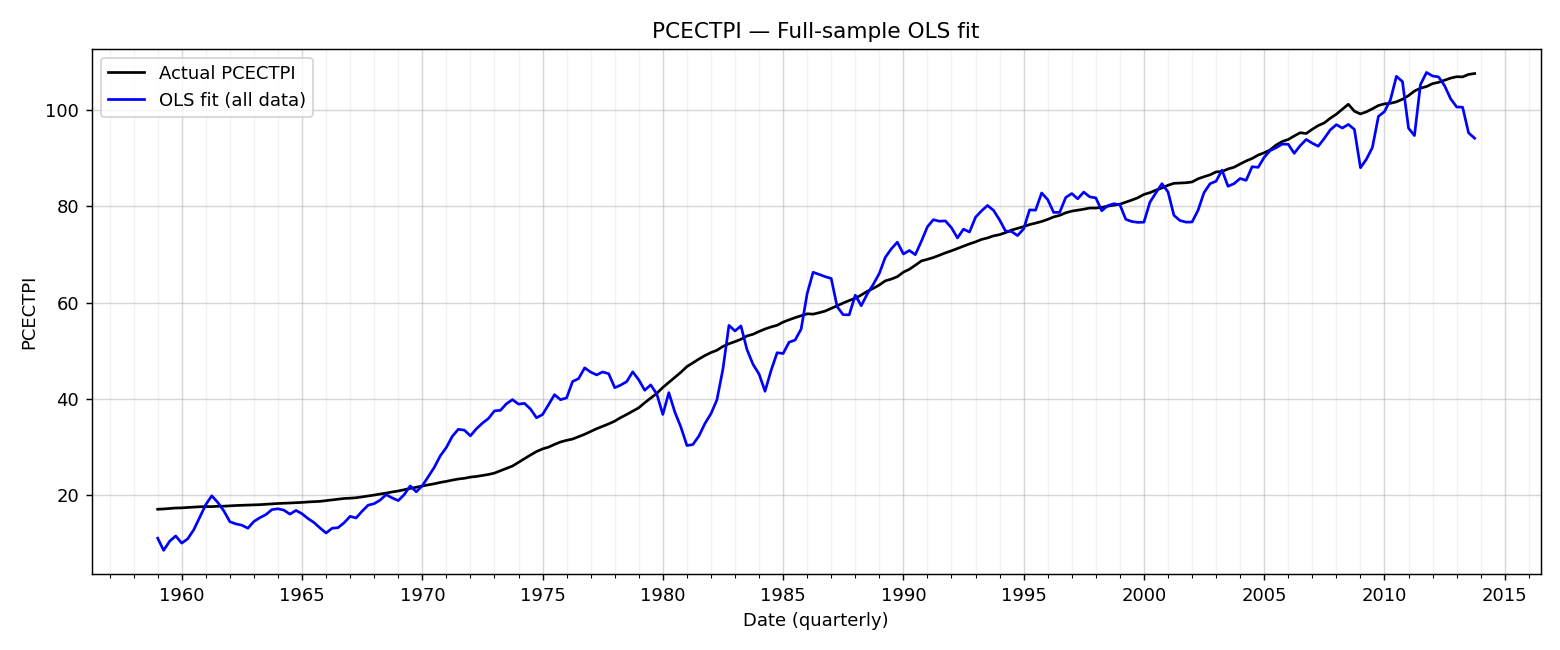
\includegraphics[width=\textwidth]{Q1_full_fit.png}
     \caption{PCECTPI full-sample OLS fit. Actual series in black, fitted values in blue. Sparse year-tick formatting is applied so the x-axis is legible.}
     \label{fig:q1_fullfit}
\end{figure}

\begin{figure}[H]
     \centering
     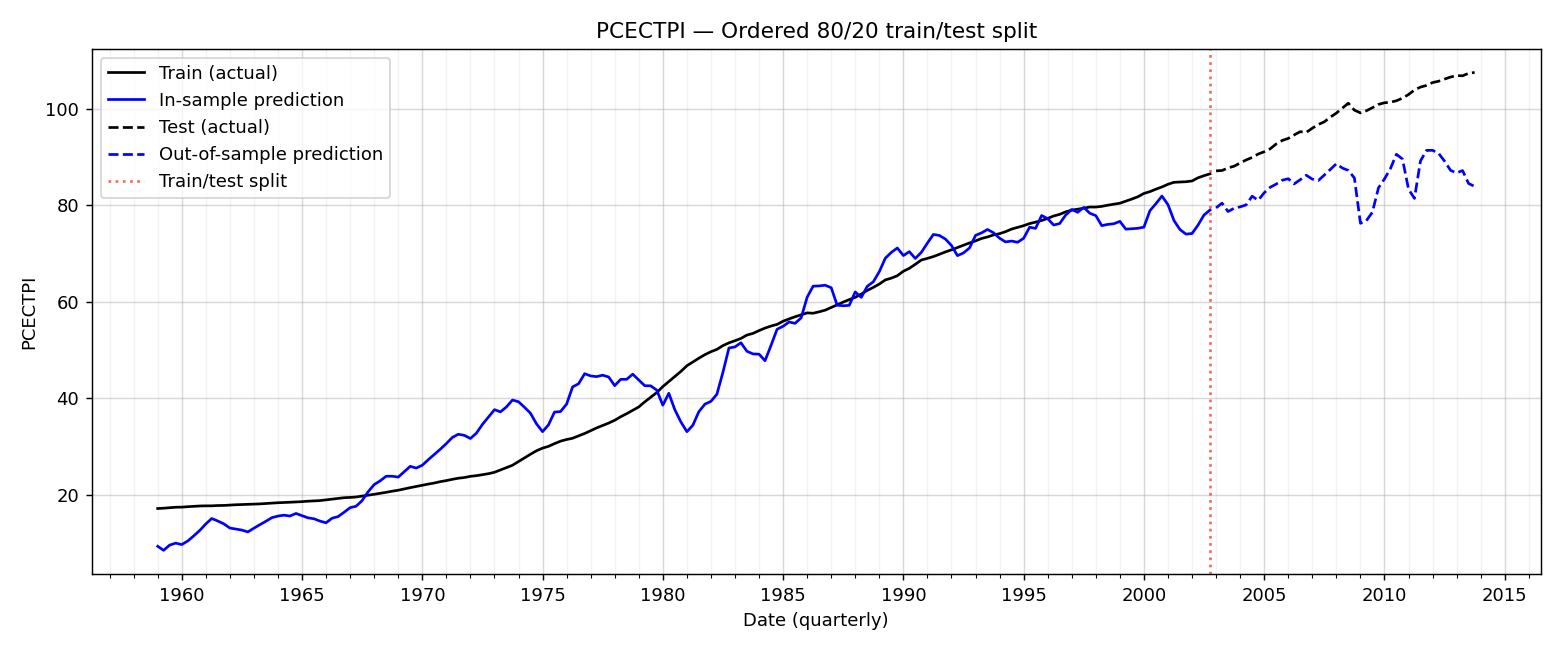
\includegraphics[width=\textwidth]{Q1_train_test.png}
     \caption{PCECTPI ordered 80/20 train/test split. Solid lines are the first 176 quarters (training), dashed lines are the remaining 44 quarters (test). The red dotted line marks the split. The out-of-sample predictions (blue dashed) clearly under-shoot the actuals (black dashed) in the post-2002 window.}
     \label{fig:q1_traintest}
\end{figure}

\end{homeworkProblem}
\pagebreak

% ==========================================
% QUESTION 2
% ==========================================
\begin{homeworkProblem}

\textbf{Run the code shared in the ``GLM.py'' file for the \texttt{chip\_dataset.csv} data: [Points 50]}
\begin{itemize}
    \item Explain the model summary when the entire data is fitted. Discuss R-squared, Df Residuals, Df Model, Method, F-statistic, Prob (F-statistic), Log-Likelihood, AIC, BIC, Coef, Std err, t, and $P > |t|$.
    \item Run with the train-test split when the order is not important and compare the results of the test with the above model fitted on the entire data.
    \item Run all three variations of ANOVA and discuss results on SSR, df\_diff, ss\_diff, df\_resid, F and $\Pr(>F)$.
    \item Submit appropriately labeled visuals.
\end{itemize}

The target is \texttt{FP32 GFLOPS\_Target}, the single-precision floating-point throughput of the chip. The regressors are the five hardware specifications. After \texttt{sm.add\_constant} the layout is $\beta_0 = $ const, $\beta_1 = $ \texttt{Process Size (nm)} (\texttt{x1}), $\beta_2 = $ \texttt{TDP (W)} (\texttt{x2}), $\beta_3 = $ \texttt{Die Size (mm\^{}2)} (\texttt{x3}), $\beta_4 = $ \texttt{Transistors (million)} (\texttt{x4}), $\beta_5 = $ \texttt{Freq (MHz)} (\texttt{x5}). The dataset has $1{,}610$ rows and no missing values.

\hrulefill

\subsection*{Part a) Full-Sample OLS Summary}

\begin{lstlisting}[language=Python, title={Python Console Output: Full-Sample OLS Summary}]
                            OLS Regression Results
==============================================================================
Dep. Variable:                      y   R-squared:                       0.790
Model:                            OLS   Adj. R-squared:                  0.790
Method:                 Least Squares   F-statistic:                     1210.
Date:                Fri, 10 Apr 2026   Prob (F-statistic):               0.00
Time:                        17:54:09   Log-Likelihood:                -14449.
No. Observations:                1610   AIC:                         2.891e+04
Df Residuals:                    1604   BIC:                         2.894e+04
Df Model:                           5
Covariance Type:            nonrobust
==============================================================================
                 coef    std err          t      P>|t|      [0.025      0.975]
------------------------------------------------------------------------------
const      -2686.9596    254.004    -10.578      0.000   -3185.175   -2188.744
x1             3.2061      3.613      0.887      0.375      -3.880      10.292
x2             2.7005      0.732      3.687      0.000       1.264       4.137
x3             1.5224      0.550      2.768      0.006       0.443       2.601
x4             0.4985      0.014     35.369      0.000       0.471       0.526
x5             3.2043      0.210     15.230      0.000       2.792       3.617
==============================================================================
\end{lstlisting}

\textbf{Discussion of each summary statistic:}
\begin{itemize}
    \item \textbf{Method = Least Squares.} Same closed-form OLS estimator as Q1.
    \item \textbf{No. Observations = 1610, Df Model = 5, Df Residuals = 1604.} Five hardware regressors plus an intercept, leaving $1610 - 6 = 1604$ residual degrees of freedom.
    \item \textbf{R-squared = 0.790, Adj. R-squared = 0.790.} The five hardware attributes explain $79\%$ of the variance in \texttt{FP32 GFLOPS}. The gap between R-squared and Adjusted R-squared is negligible at this sample size.
    \item \textbf{F-statistic = 1210, Prob(F-statistic) $\approx$ 0.00.} The joint null of all-zero slopes is rejected by a massive margin. The hardware specs as a block have extremely high explanatory power.
    \item \textbf{Log-Likelihood = $-14{,}449$.} Not interpretable in isolation, only via model comparison.
    \item \textbf{AIC = 28{,}910, BIC = 28{,}942.} Both are large in absolute terms because of the very large residual variance (FP32 GFLOPS spans several orders of magnitude), but are still informative for comparison with nested sub-models.
    \item \textbf{Coef / Std err / t / P>|t|.} Four of the five regressors are significant at $\alpha = 0.05$. \texttt{Transistors (million)} dominates with $t = 35.37$, as one would expect since chip performance is fundamentally driven by transistor count, followed by \texttt{Freq (MHz)} ($t = 15.23$). \texttt{Process Size (nm)} is \textbf{not significant} ($p = 0.375$). Once transistor count, clock frequency, and die size are in the model, the nanometre process node contributes no additional information. The intercept is large and negative because the fitted plane is extrapolating far outside the observed range of specs.
    \item \textbf{Condition number $\approx 3.59 \times 10^{4}$.} Flagged by statsmodels as a possible multicollinearity issue, which is plausible because transistor count and die size are strongly correlated in practice.
\end{itemize}

\subsection*{Part b) Random 80/20 Train-Test Split}

Chip rows are independent hardware products, not a time series, so we use the scikit-learn random split with \texttt{random\_state=42}, matching \texttt{GLM.py}. Train size: $1{,}288$. Test size: $322$.

\vspace{0.5em}
\begin{center}
\begin{tabular}{lrrrrrr}
\toprule
\textbf{Model} & $R^2$ & \textbf{Adj $R^2$} & \textbf{AIC} & \textbf{BIC} & \textbf{In-sample RMSE} & \textbf{Test RMSE} \\
\midrule
Full-sample (all 1610) & 0.7905 & 0.7898 & 28909.5454 & 28941.8493 & 1911.1385 & n/a \\
Train-only (80\%)      & 0.7904 & 0.7896 & 23118.4927 & 23149.4577 & 1902.5935 & 1949.7451 \\
\bottomrule
\end{tabular}
\end{center}
\vspace{0.5em}

\begin{lstlisting}[language=Python, title={Python Console Output: Train-Only OLS Summary}]
                            OLS Regression Results
==============================================================================
Dep. Variable:                      y   R-squared:                       0.790
Model:                            OLS   Adj. R-squared:                  0.790
Method:                 Least Squares   F-statistic:                     966.7
Date:                Fri, 10 Apr 2026   Prob (F-statistic):               0.00
Time:                        17:54:10   Log-Likelihood:                -11553.
No. Observations:                1288   AIC:                         2.312e+04
Df Residuals:                    1282   BIC:                         2.315e+04
Df Model:                           5
Covariance Type:            nonrobust
==============================================================================
                 coef    std err          t      P>|t|      [0.025      0.975]
------------------------------------------------------------------------------
const      -2662.6614    287.560     -9.260      0.000   -3226.801   -2098.522
x1             2.0991      4.027      0.521      0.602      -5.801       9.999
x2             2.4700      0.809      3.054      0.002       0.883       4.057
x3             1.8139      0.620      2.927      0.003       0.598       3.030
x4             0.4842      0.015     31.343      0.000       0.454       0.515
x5             3.1989      0.237     13.491      0.000       2.734       3.664
==============================================================================
\end{lstlisting}

\textbf{Conclusion:}\\
Unlike the time-series case in Q1, the train-only and full-sample fits are virtually identical: $R^2 = 0.7904$ vs. $0.7905$, and the test RMSE ($1949.7$) is within $2.5\%$ of the in-sample RMSE ($1902.6$). Because the random 80/20 split samples chips uniformly from the whole dataset, there is no distribution shift between train and test, and the held-out predictions generalise cleanly. \texttt{Process Size} stays insignificant in the train-only fit ($p = 0.602$), further confirming it is not useful even after re-sampling.

\subsection*{Part c) Three Variations of ANOVA}

\begin{lstlisting}[language=Python, title={Python Console Output: ANOVA 1 -- Full vs Intercept-Only}]
========================================================================
ANOVA 1 -- Full model vs Intercept-only (null) model
========================================================================
   df_resid           ssr  df_diff       ss_diff            F  Pr(>F)
0    1609.0  2.806695e+10      0.0           NaN          NaN     NaN
1    1604.0  5.880445e+09      5.0  2.218651e+10  1210.355874     0.0
\end{lstlisting}

\begin{lstlisting}[language=Python, title={Python Console Output: ANOVA 2 -- Reduced (Process Size, TDP, Freq) vs Full}]
========================================================================
ANOVA 2 -- Reduced (const, Process Size, TDP, Freq) vs Full
========================================================================
   df_resid           ssr  df_diff       ss_diff            F         Pr(>F)
0    1606.0  1.400884e+10      0.0           NaN          NaN            NaN
1    1604.0  5.880445e+09      2.0  8.128393e+09  1108.584626  4.492497e-303
\end{lstlisting}

\begin{lstlisting}[language=Python, title={Python Console Output: ANOVA 3 -- Full vs Itself}]
========================================================================
ANOVA 3 -- Full model vs itself
========================================================================
   df_resid           ssr  df_diff  ss_diff   F  Pr(>F)
0    1604.0  5.880445e+09      0.0      NaN NaN     NaN
1    1604.0  5.880445e+09     -0.0     -0.0 NaN     NaN
\end{lstlisting}

\textbf{Discussion:}
\begin{itemize}
    \item \textbf{ANOVA 1.}\\
    Compares the full model to the intercept-only null. The null residual sum of squares is $2.807 \times 10^{10}$, and adding the five regressors drops it to $5.88 \times 10^{9}$, an extra sum of squares of $\mathrm{ss\_diff} = 2.22 \times 10^{10}$ with $\mathrm{df\_diff} = 5$. $F = 1210.36$, $p \approx 0$, identical to the headline F in \texttt{summary()}. The joint null of all-zero slopes is decisively rejected.

    \item \textbf{ANOVA 2.}\\
    Compares a reduced ``spec-sheet'' model containing only (const, \texttt{Process Size}, \texttt{TDP}, \texttt{Freq}) against the full model. The reduced $\mathrm{SSR} = 1.401 \times 10^{10}$ drops to $5.88 \times 10^{9}$ in the full model, and the extra sum of squares from adding \texttt{Die Size} and \texttt{Transistors} is $\mathrm{ss\_diff} = 8.13 \times 10^{9}$, paid for with $\mathrm{df\_diff} = 2$ additional parameters. $F = 1108.58$, $p = 4.5 \times 10^{-303}$. Adding die size and transistor count is overwhelmingly significant. Headline clock speed and TDP are not enough on their own, and the silicon area and transistor budget carry independent information about throughput.

    \item \textbf{ANOVA 3.}\\
    Compares the full model to itself. $\mathrm{ss\_diff} = 0$, $\mathrm{df\_diff} = 0$, $F = \texttt{NaN}$. A structural sanity check only.
\end{itemize}

\subsection*{Part d) Visuals}

\begin{figure}[H]
     \centering
     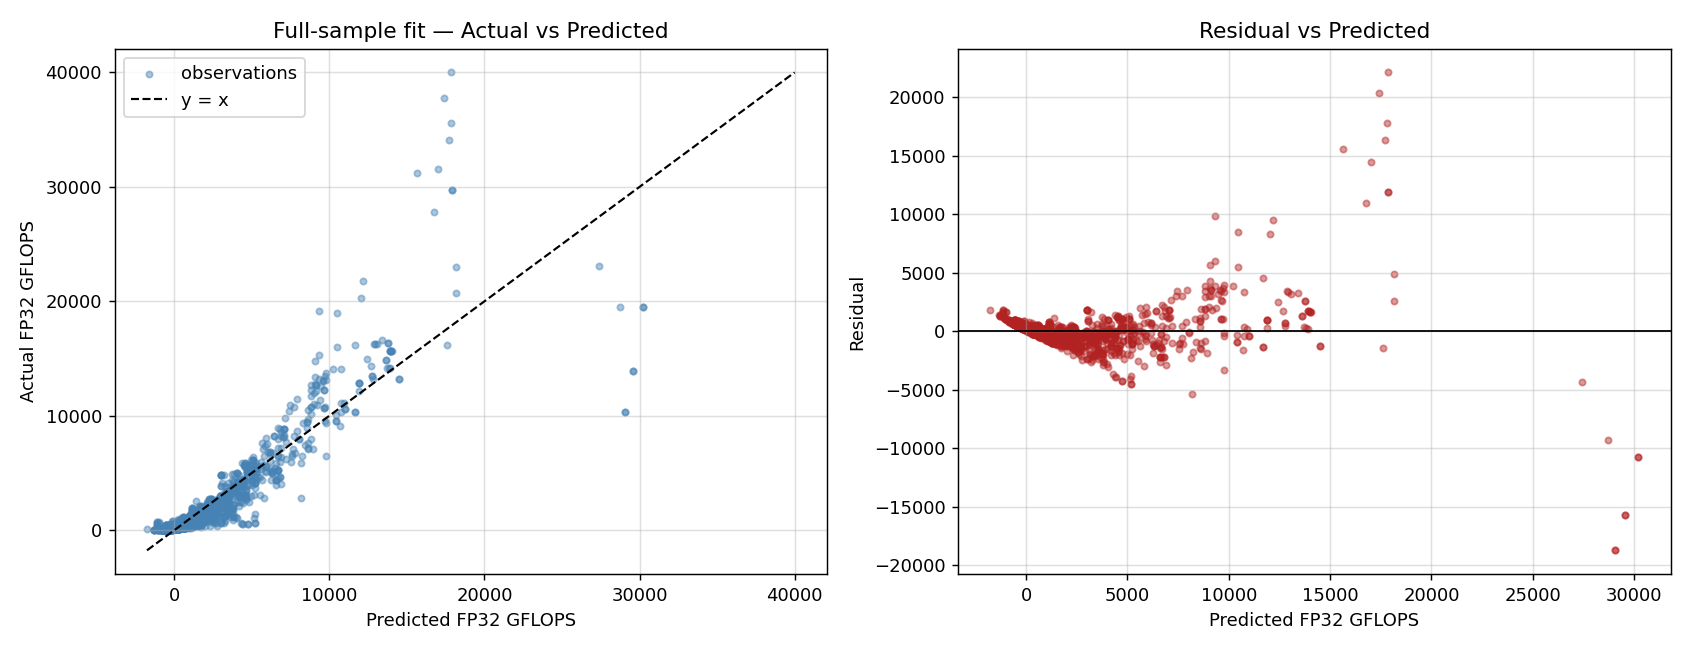
\includegraphics[width=\textwidth]{Q2_full_fit.png}
     \caption{Chip dataset full-sample OLS fit. Left: actual vs predicted \texttt{FP32 GFLOPS} with the $y = x$ line. Right: residuals vs. fitted values. The funnel shape in the residuals and the two or three extreme outliers are consistent with the large kurtosis (55) and skew (1.8) reported by the summary.}
     \label{fig:q2_fullfit}
\end{figure}

\begin{figure}[H]
     \centering
     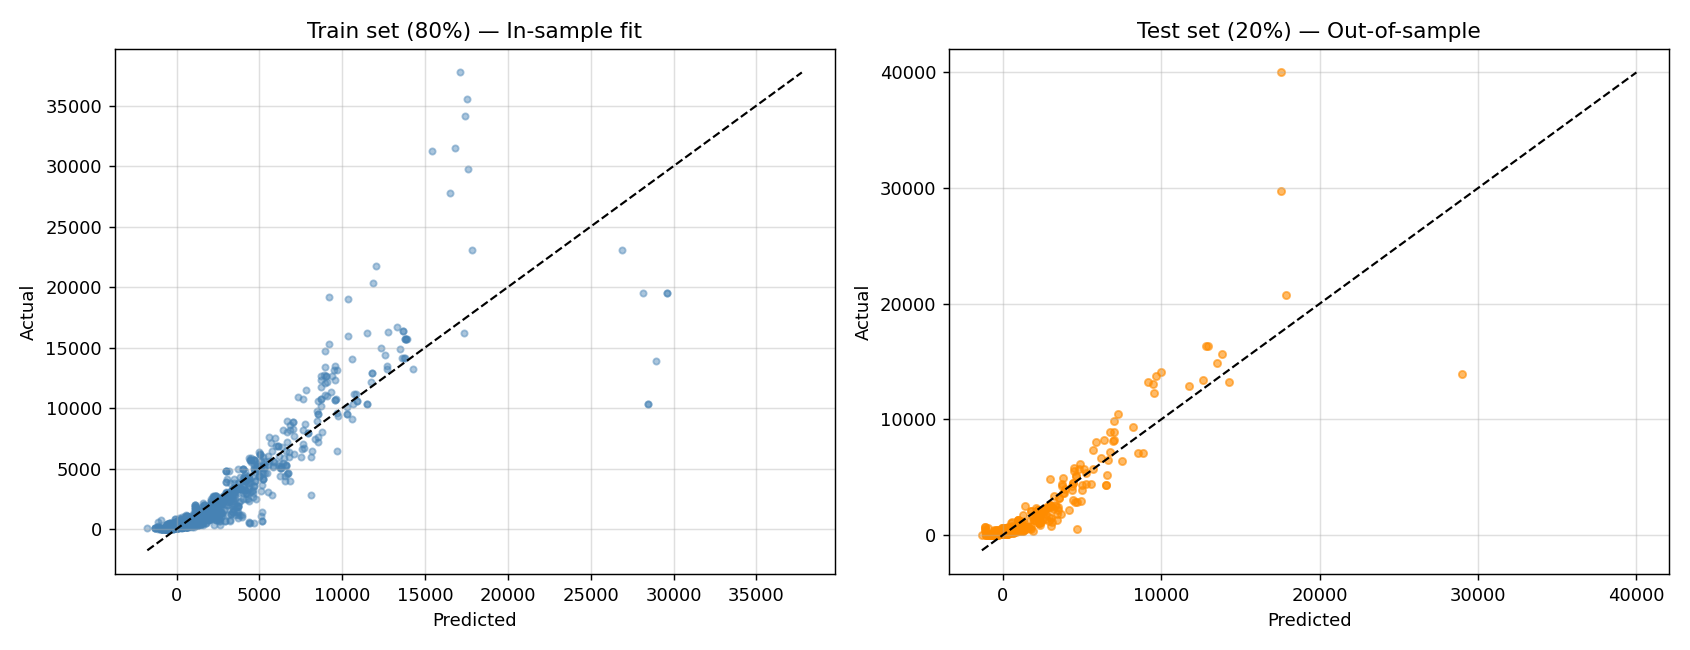
\includegraphics[width=\textwidth]{Q2_train_test.png}
     \caption{Chip dataset random 80/20 train/test split (\texttt{random\_state=42}). Left: in-sample fit on $1{,}288$ training rows. Right: out-of-sample fit on the $322$ held-out rows. The scatter patterns are almost indistinguishable, confirming the random split does not induce distribution shift.}
     \label{fig:q2_traintest}
\end{figure}

\end{homeworkProblem}
\pagebreak

% ==========================================
% QUESTION 3
% ==========================================
\begin{homeworkProblem}

\textbf{Run the code: GLM using Poisson Regression on the \texttt{Smokers\_Age.xlsx} data. And discuss the summary results. [Points 20]}

\hrulefill

\subsection*{Model}

\texttt{Deaths} is a count and therefore unsuitable for ordinary linear regression. We fit a Poisson GLM with a log link, following \texttt{GLM.py} exactly. Note that \texttt{PersonYears} is log-transformed in place so that its coefficient acts as an exposure offset:
$$
\log \mathbb{E}[\text{Deaths}_i] \;=\; \beta_0 + \beta_1 \text{Agecat}_i + \beta_2 \text{Smoke}_i + \beta_3 \text{Agecatsq}_i + \beta_4 \text{Smokeage}_i + \beta_5 \log(\text{PersonYears}_i).
$$

\subsection*{Part a) Poisson GLM Summary}

\begin{lstlisting}[language=Python, title={Python Console Output: Poisson GLM Summary}]
                 Generalized Linear Model Regression Results
==============================================================================
Dep. Variable:                 Deaths   No. Observations:                   10
Model:                            GLM   Df Residuals:                        4
Model Family:                 Poisson   Df Model:                            5
Link Function:                    Log   Scale:                          1.0000
Method:                          IRLS   Log-Likelihood:                -28.260
Date:                Fri, 10 Apr 2026   Deviance:                       1.4517
Time:                        17:54:10   Pearson chi2:                     1.39
No. Iterations:                     6   Pseudo R-squ. (CS):              1.000
Covariance Type:            nonrobust
===============================================================================
                  coef    std err          z      P>|z|      [0.025      0.975]
-------------------------------------------------------------------------------
Intercept      -8.7447      4.803     -1.821      0.069     -18.158       0.669
Agecat          2.3927      0.213     11.250      0.000       1.976       2.810
Smoke           1.7785      0.877      2.029      0.042       0.060       3.497
Agecatsq       -0.2210      0.061     -3.614      0.000      -0.341      -0.101
Smokeage       -0.3129      0.099     -3.150      0.002      -0.508      -0.118
PersonYears     0.7837      0.506      1.550      0.121      -0.207       1.775
===============================================================================
\end{lstlisting}

\subsection*{Part b) Incidence-Rate Ratios}

Because the link is $\log$, exponentiating each coefficient gives an \emph{Incidence-Rate Ratio} (IRR), the multiplicative change in the expected death rate per unit change in the regressor.

\vspace{0.5em}
\begin{center}
\begin{tabular}{lrrrrrc}
\toprule
\textbf{Parameter} & \textbf{Coef} & \textbf{Std err} & \textbf{z} & \textbf{P>|z|} & \textbf{IRR = exp(Coef)} & \textbf{Sig. at 0.05} \\
\midrule
Intercept    & $-8.7447$ & $4.8029$ & $-1.8207$ & $0.0687$ & $0.000159$ & No  \\
Agecat       & $2.3927$  & $0.2127$ & $11.2503$ & $0.0000$ & $10.9427$  & Yes \\
Smoke        & $1.7785$  & $0.8766$ & $2.0289$  & $0.0425$ & $5.9210$   & Yes \\
Agecatsq     & $-0.2210$ & $0.0612$ & $-3.6140$ & $0.0003$ & $0.8017$   & Yes \\
Smokeage     & $-0.3129$ & $0.0993$ & $-3.1500$ & $0.0016$ & $0.7313$   & Yes \\
PersonYears  & $0.7837$  & $0.5057$ & $1.5498$  & $0.1212$ & $2.1895$   & No  \\
\bottomrule
\end{tabular}
\end{center}
\vspace{0.5em}

\subsection*{Discussion of the summary results}

\begin{itemize}
    \item \textbf{Model family / link / method.}\\
    \texttt{Poisson} with \texttt{Log} link, fitted by IRLS (Iteratively Reweighted Least Squares), converged in $6$ iterations.

    \item \textbf{No. Observations = 10, Df Model = 5, Df Residuals = 4.}\\
    Only ten rows are available (five age-categories $\times$ two smoker strata), leaving four residual degrees of freedom. Statistical power is inherently limited on this dataset.

    \item \textbf{Deviance = 1.4517 on 4 df.}\\
    The ratio $\text{Deviance}/\text{df\_resid} = 0.363$ is well below $1$, so there is \textbf{no evidence of overdispersion}. The Poisson variance assumption ($\operatorname{Var} = \operatorname{E}$) holds, and a Negative Binomial extension is not needed.

    \item \textbf{Pearson chi-squared = 1.39.}\\
    Also well below the residual df, tells the same story.

    \item \textbf{Log-Likelihood = $-28.26$, AIC = $68.52$.}\\
    These are only meaningful for comparison with alternative specifications.

    \item \textbf{Intercept ($\beta_0 = -8.74$, $p = 0.069$).}\\
    Not significant at $\alpha = 0.05$. It represents the log expected death count when every predictor is zero, which is an extrapolation outside the data range.

    \item \textbf{Agecat ($\beta_1 = 2.39$, IRR $\approx 10.94$, $p < 0.001$).}\\
    Each unit increase in the age-category index multiplies the expected death rate by roughly $\mathbf{10.94}\times$, before the quadratic correction. Easily the strongest effect in the model.

    \item \textbf{Agecatsq ($\beta_3 = -0.22$, IRR $\approx 0.80$, $p < 0.001$).}\\
    Highly significant \emph{negative} quadratic correction. Together with \texttt{Agecat}, this implies that the death rate grows very steeply with age in the young cohorts but the growth rate attenuates as cohorts get older.

    \item \textbf{Smoke ($\beta_2 = 1.78$, IRR $\approx 5.92$, $p = 0.042$).}\\
    At the baseline age ($\text{Agecat} = 0$), smokers have a death rate $\mathbf{5.92}\times$ higher than non-smokers. Significant at $\alpha = 0.05$.

    \item \textbf{Smokeage ($\beta_4 = -0.31$, IRR $\approx 0.73$, $p = 0.002$).}\\
    Negative interaction: the smoker vs. non-smoker gap \emph{shrinks} with age, because at older ages non-smokers catch up to smokers in absolute mortality risk. The relative risk of smoking is highest in middle-aged cohorts, consistent with the public-health literature.

    \item \textbf{PersonYears ($\beta_5 = 0.78$, $p = 0.121$).}\\
    Not significant. In a textbook exposure-offset setup this coefficient would be fixed at exactly $1$ (via \texttt{statsmodels}'s \texttt{offset=} argument). Because \texttt{GLM.py} enters $\log(\text{PersonYears})$ as an ordinary regressor instead, the model is allowed to estimate it freely, and with only $10$ observations and $5$ other regressors it cannot pin it down with any precision. The point estimate of $0.78$ is not statistically distinguishable from either $0$ or $1$, so the exposure-offset interpretation is not contradicted.
\end{itemize}

\subsection*{Visual}

\begin{figure}[H]
     \centering
     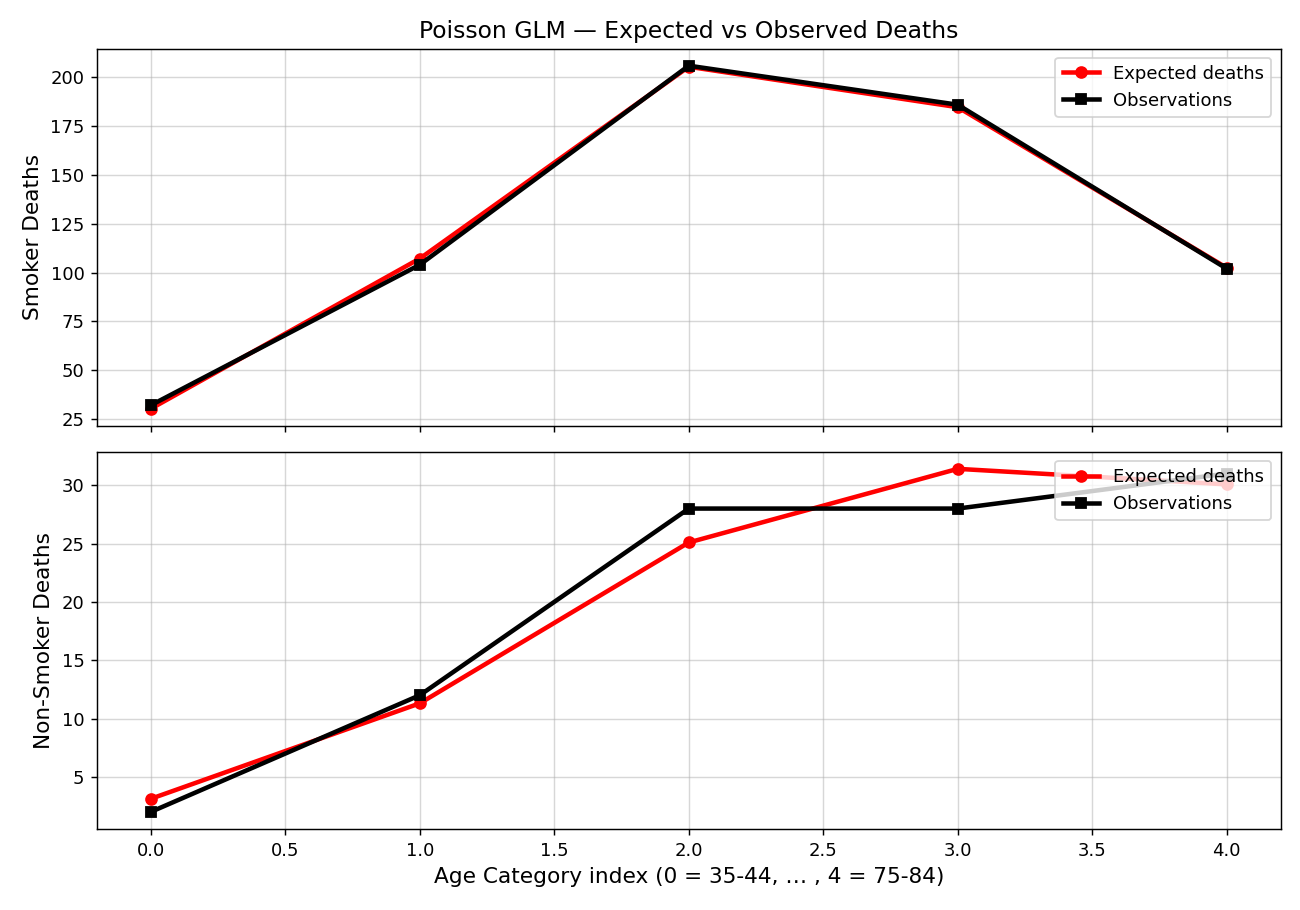
\includegraphics[width=0.85\textwidth]{Q3_smokers_poisson.png}
     \caption{Poisson GLM expected vs observed deaths by age category. Top panel: smokers. Bottom panel: non-smokers. The fitted curves (red) track the observed counts (black) very closely in both strata, consistent with the low deviance and Pearson $\chi^2$ reported above.}
     \label{fig:q3_poisson}
\end{figure}

\subsection*{Overall Conclusion}

\textbf{Conclusion:}\\
The Poisson GLM fits the mortality data very well: deviance and Pearson $\chi^2$ are both below their residual degrees of freedom, and the fitted curves hug the observed deaths in both smoker and non-smoker strata. The four covariates with interpretable biology, \texttt{Agecat}, \texttt{Agecatsq}, \texttt{Smoke}, and \texttt{Smokeage}, are all statistically significant at $\alpha = 0.05$, and their signs match the public-health story. Death rates rise steeply with age (with a small convex attenuation), smoking multiplies the death rate roughly six-fold at baseline age, and the smoker vs. non-smoker gap closes as both cohorts approach the end of life.

\end{homeworkProblem}

\end{document}
